\newpage
\section{Limits of \HbbVqq signals fail $\Hbb$ tagger, pass $\Hww$ tagger}
\label{results}

%\begin{figure*}[h!tpb]
%\begin{center}
%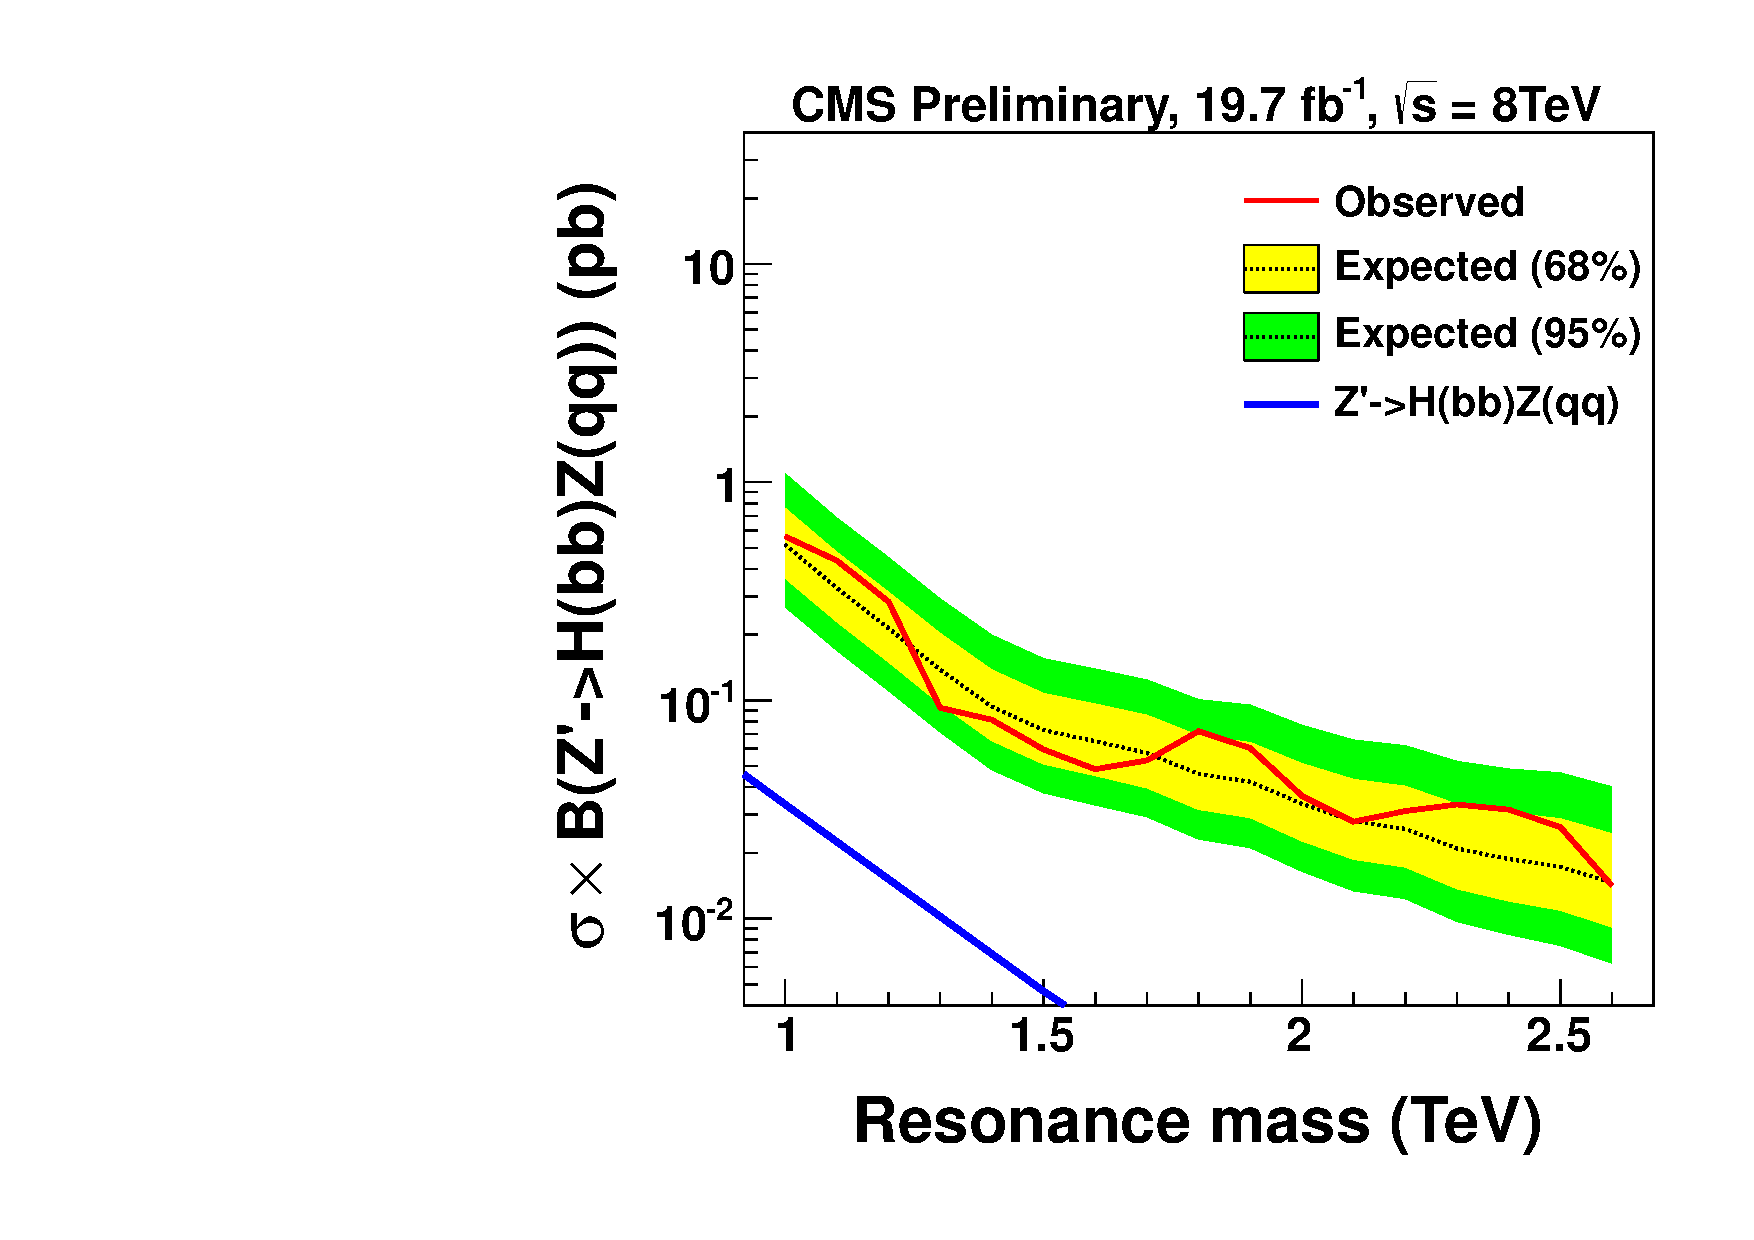
\includegraphics[width=0.49\textwidth]{HqqqqZqqfigs/HbbHww/Limits/brazilianFlag_HbbPassHww_Combine.pdf}
%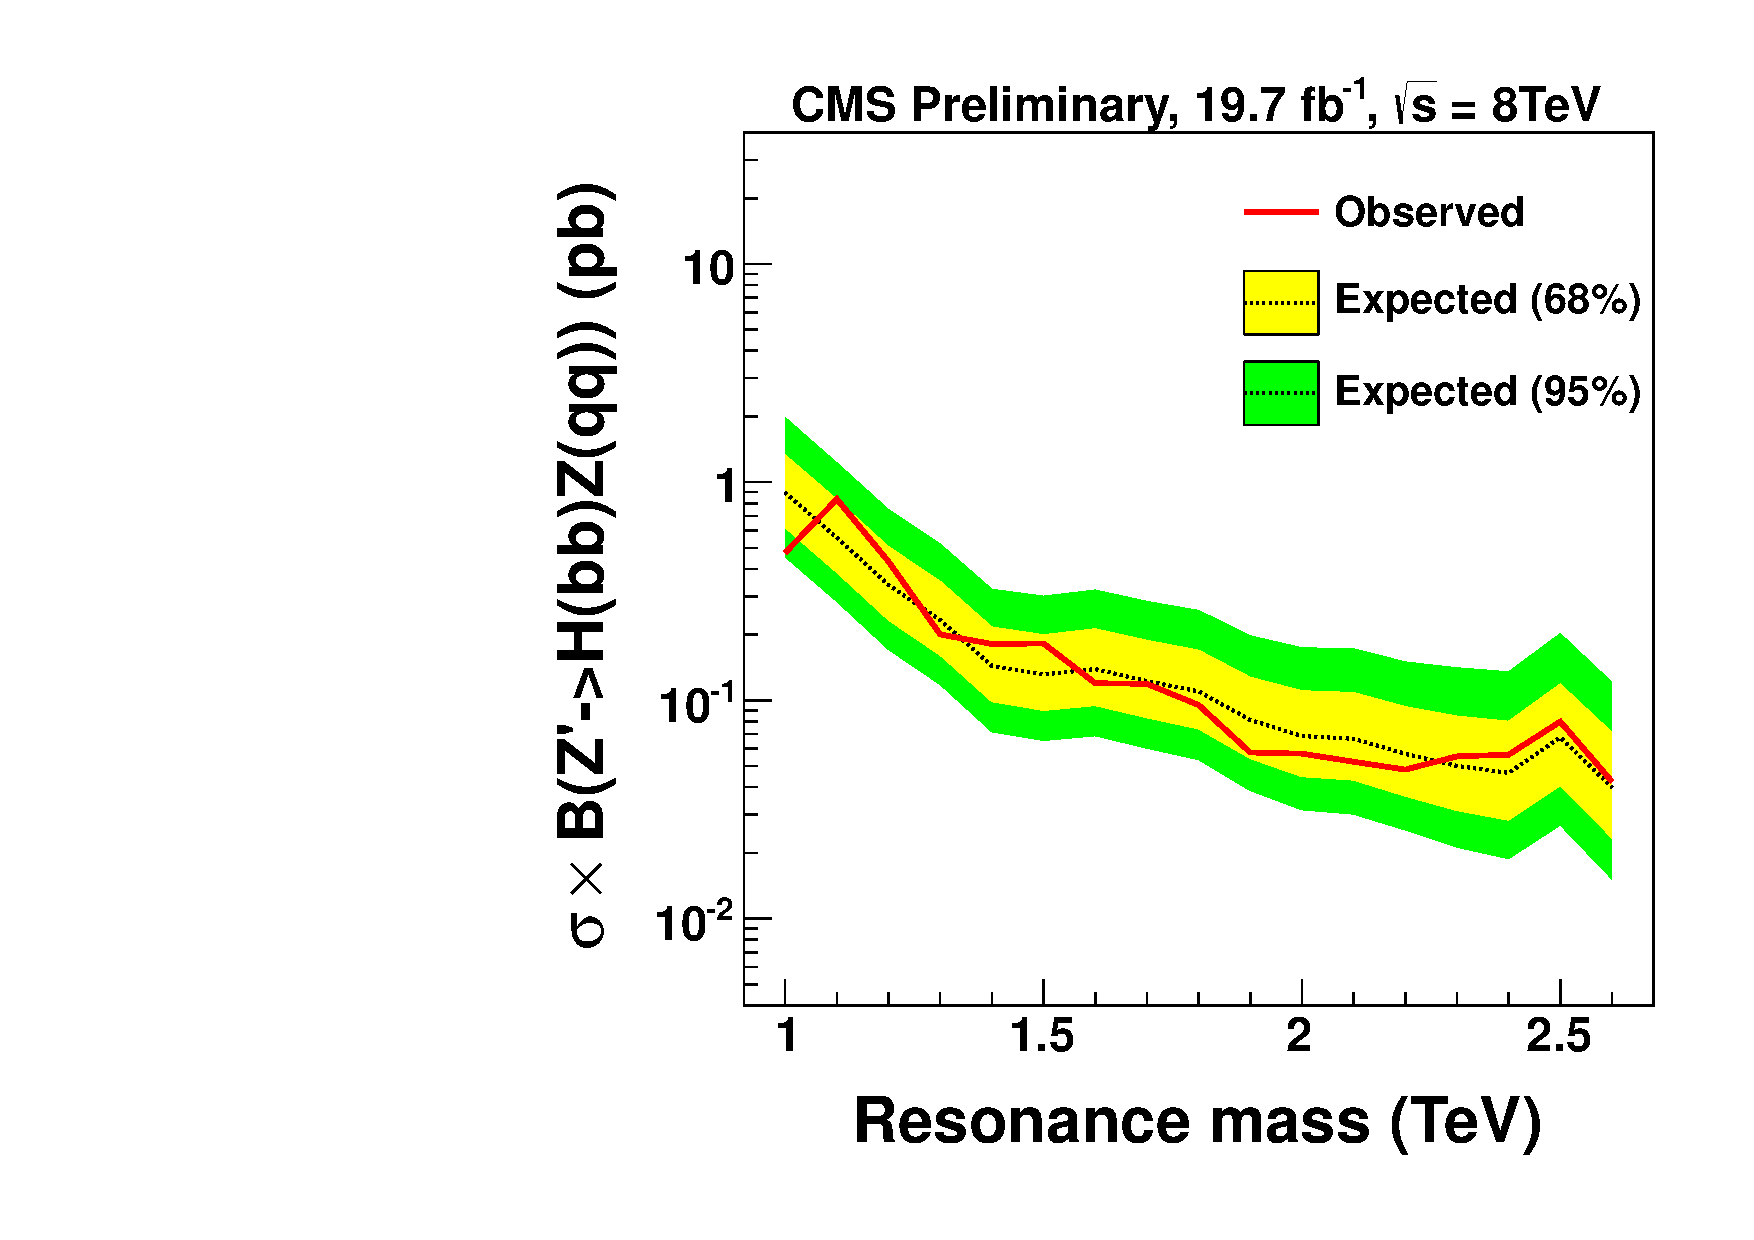
\includegraphics[width=0.49\textwidth]{HqqqqZqqfigs/HbbHww/Limits/brazilianFlag_HbbPassHww_HighPuri.pdf}
%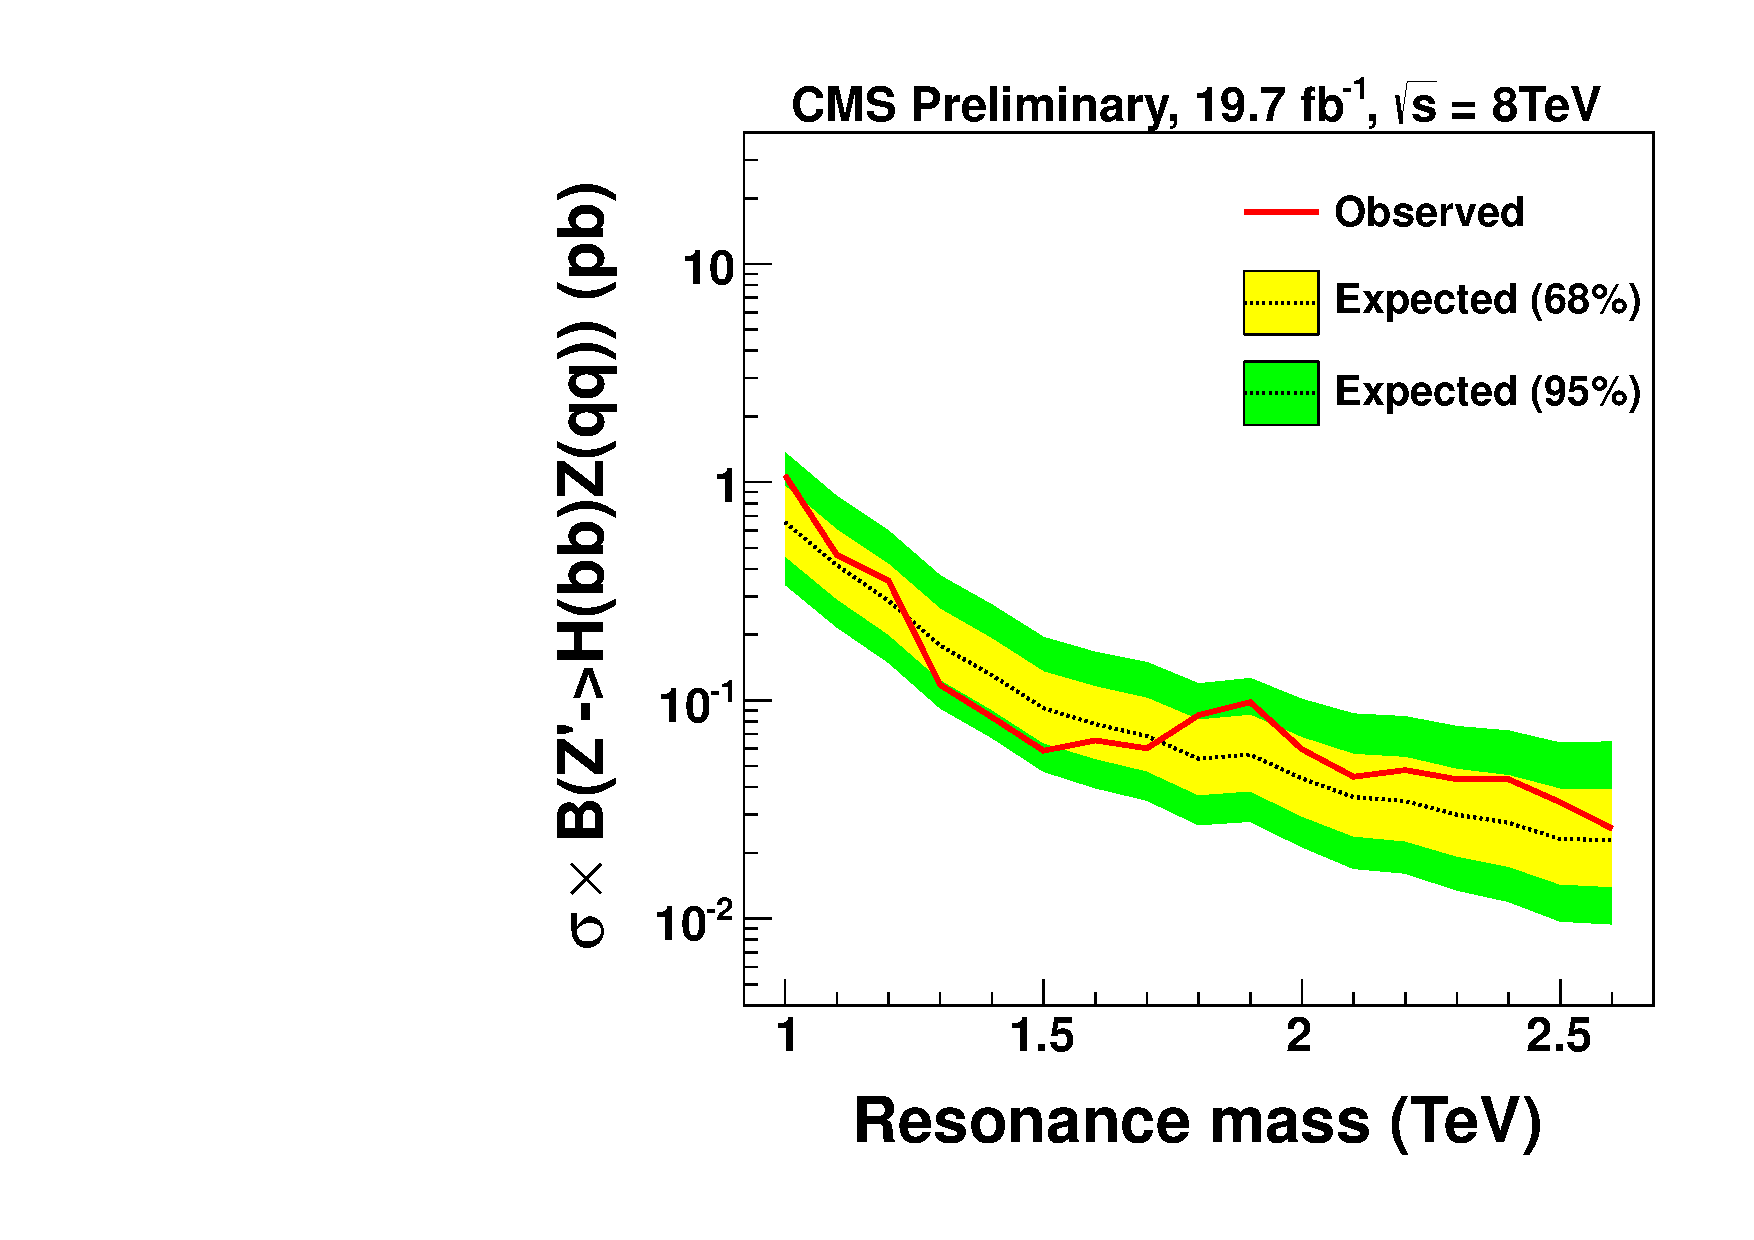
\includegraphics[width=0.49\textwidth]{HqqqqZqqfigs/HbbHww/Limits/brazilianFlag_HbbPassHww_LowH.pdf}
%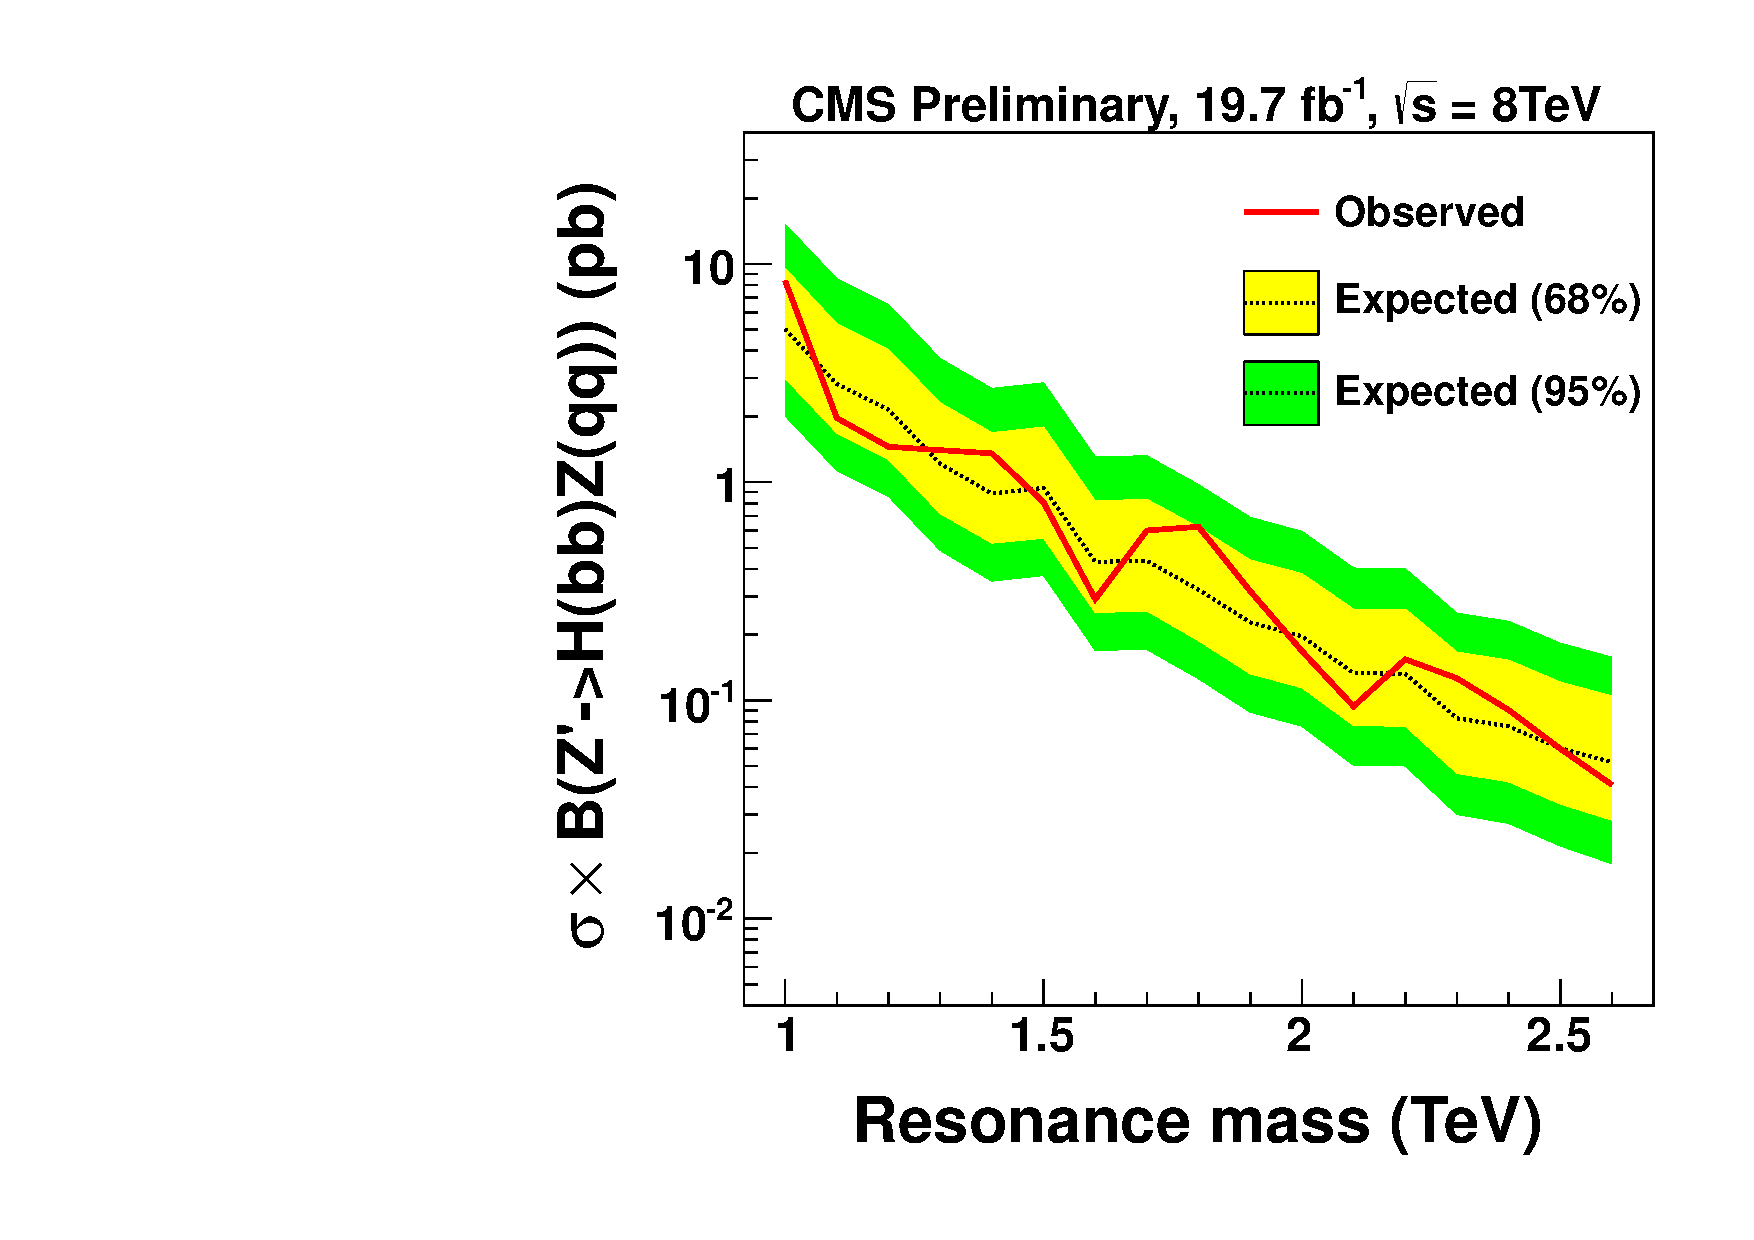
\includegraphics[width=0.49\textwidth]{HqqqqZqqfigs/HbbHww/Limits/brazilianFlag_HbbPassHww_LowV.pdf}
%\end{center}
%\caption{Expected and observed limits for H(bb)Z(qq) search. The combined limit is on top left. the high purity limit
%is the top right one. and the low purity H-tagging limit is on the bottom left. the low purity V-tagging on bottom right.   
%}
%\label{fig:HbbHwwLimits}
%\end{figure*}

Figure~\ref{fig:HbbVHwwCombined} shows the limits for \HbbVqq signals, failing the $\Hbb$ tagger , but
 passing the
$\Hww$ tagger. Limits of combining category Hww1, Hww2 and Hww3 are presented.
The $\Hbb$ and V bosons braching ratios are already taken into account.


\begin{figure}[ht!pb]
\begin{center}
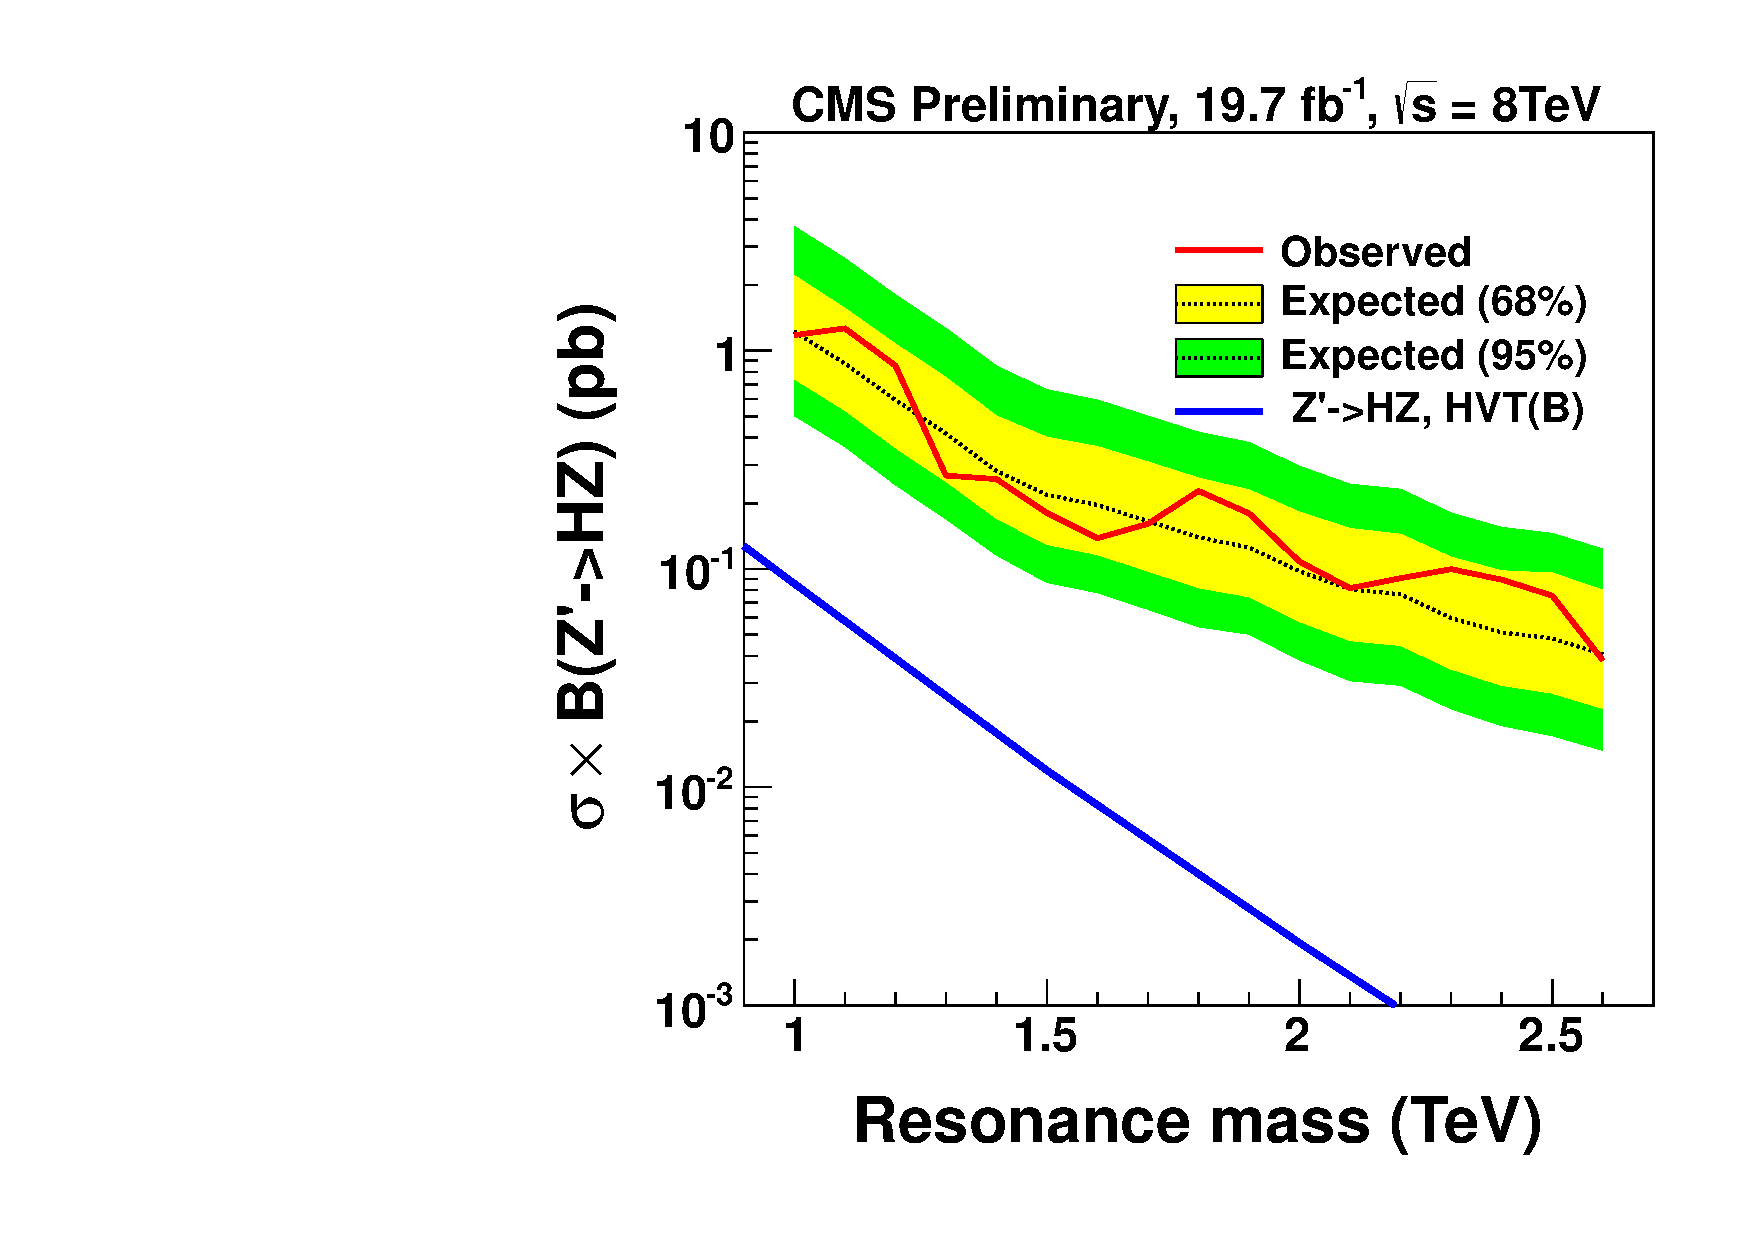
\includegraphics[width=0.49\textwidth]{EXO-14-009/brazilianFlag_HbbZqqHwwHPLPHV.pdf}
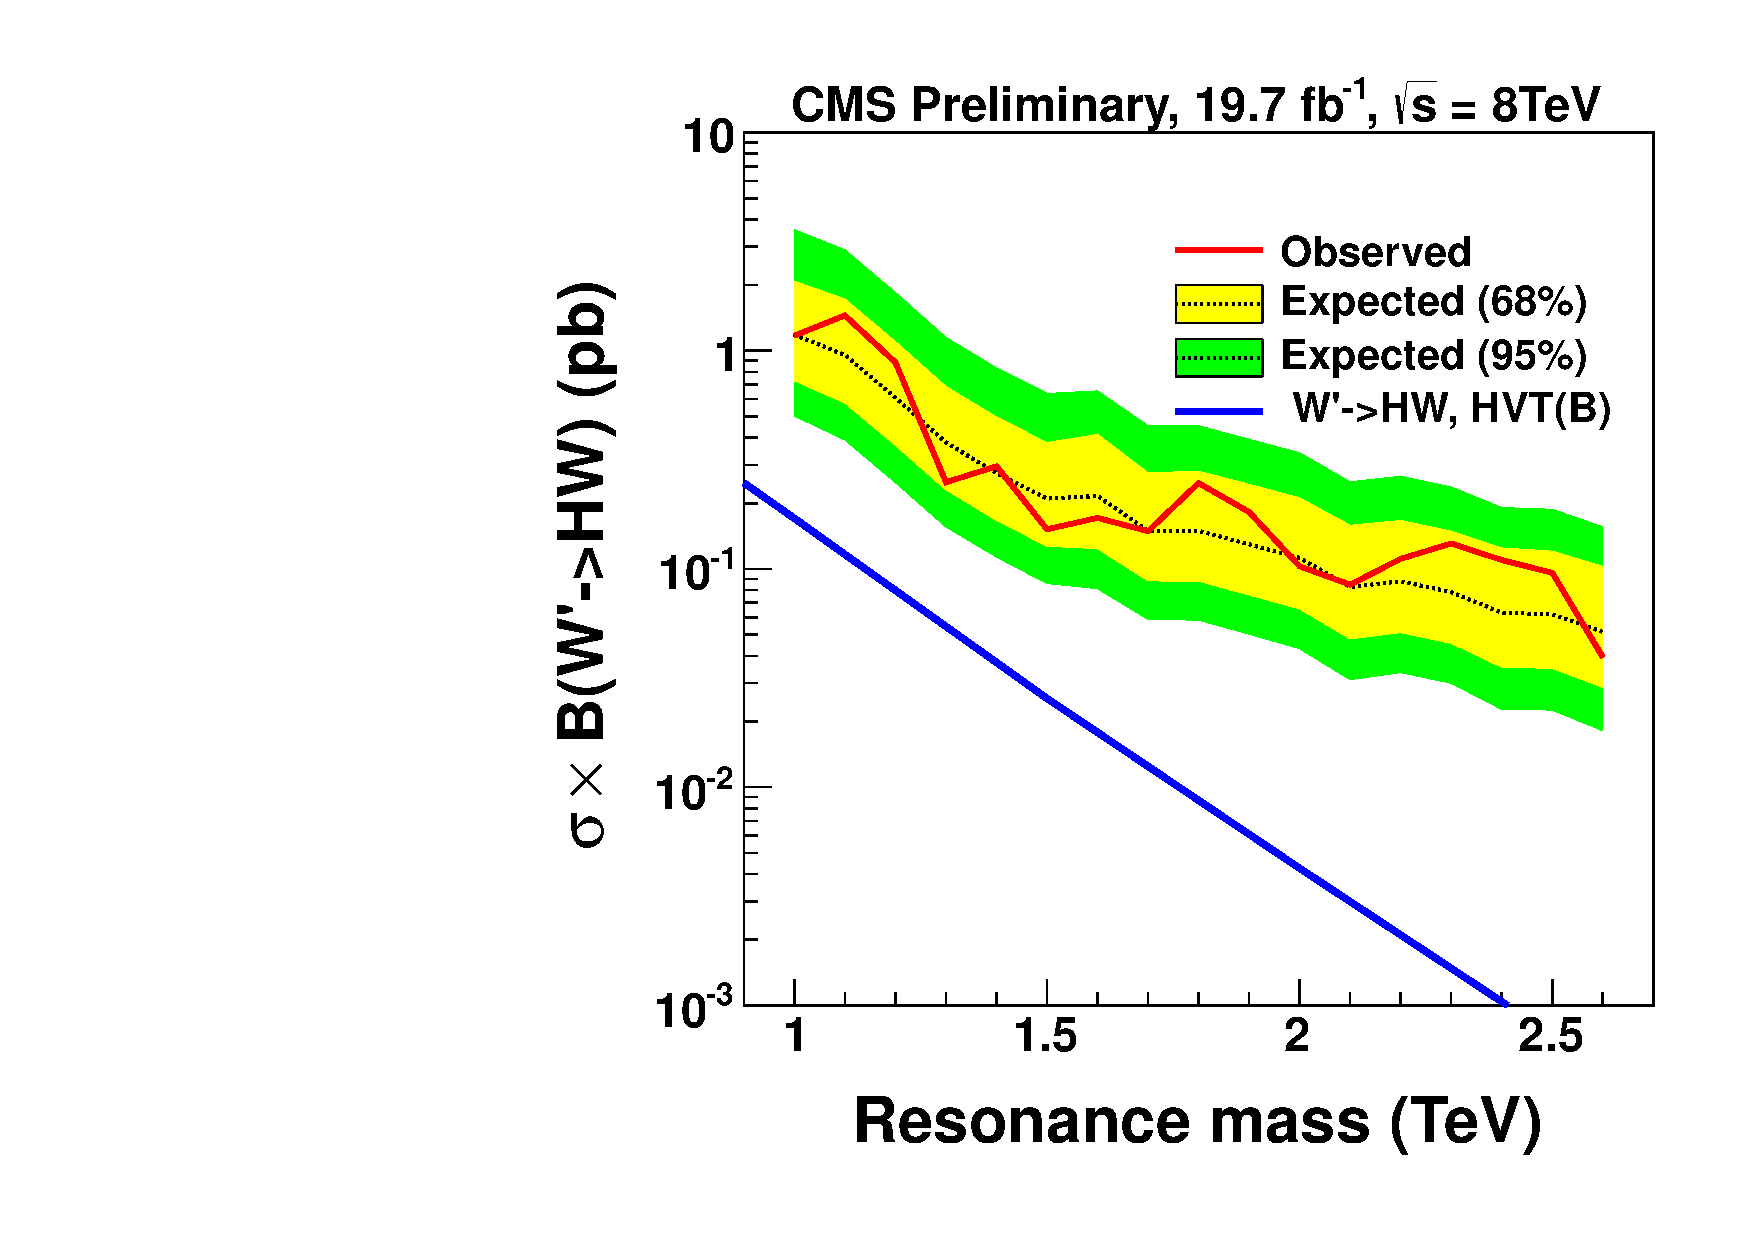
\includegraphics[width=0.49\textwidth]{EXO-14-009/brazilianFlag_HbbWqqHwwHPLPHV.pdf}
\end{center}
\caption{Expected and observed limits for ${\rm Z'\to HZ}$(left) and ${\rm W' \to WZ}$(right)
 search, in $\Hbb$ decay mode, but pass $\Hww$ tagger. Branching ratios of $\Hbb$ and V decays are
 taken into account. Theory model used here is HVT scenario B, arXiv:1402.4431.
% The high purity is on the bottom left. the low purity V-tagging on bottom right.
%  The predicted cross sections as a function of resonance mass for the considered benchmark models are overlaid.
}
\label{fig:HbbVHwwCombined}
\end{figure}




\clearpage
